\chapter{Introduction} \label{ch:introduction}

\section{Concept and Motivation}
% What are we trying to get done here?
% Humanoid robots are great, and we want to get things done with them.
% We ended up doing navigation and crawling.
Humanoid robots are a very versatile mobile platform, allowing many different
areas of research. In this thesis, the areas of navigation and crawling were
explored.
% Navigating a humanoid robot.
% Navigating a humanoid is necessary if we want to get the robot to do things
% that aren't where it already is.
% Get there to manipulate, create a map of environment, survey, etc.
Mobile platforms allow for many interesting tasks. They can be used for security
surveillance \cite{knightscope}, create maps \cite{Thrun02}, 
or deliver objects from one place to another \cite{savioke}.
To allow for these applications, robots must be able to safely traverse through
an environment. Figure~\ref{fig:nao_with_obstacle2} shows an example of this.
Development of safe and robust navigation algorithms is 
important to achieving this end.
% Crawling a humanoid robot.
% Crawling can give the robot access to places where it can't walk.
% Crawling is more stable.
% Crawling can get you under things.
% Crawling can get you over difficult terrain.
To enable navigation on legged platforms, the robot must have an effective
gaiting strategy. While walking is often explored, crawling can allow a robot
to traverse highly irregular terrain as well as reach height constrained spaces.
This broadens the set of observable areas as well as potential manipulation
targets.
% Why are we trying to get these things done?
% Navigating is a fundamental thing for mobile robots.
% Crawling gives the robot another mode of locomotion and allows it to get to
% more places.

\begin{figure}[h!]
	\centering
    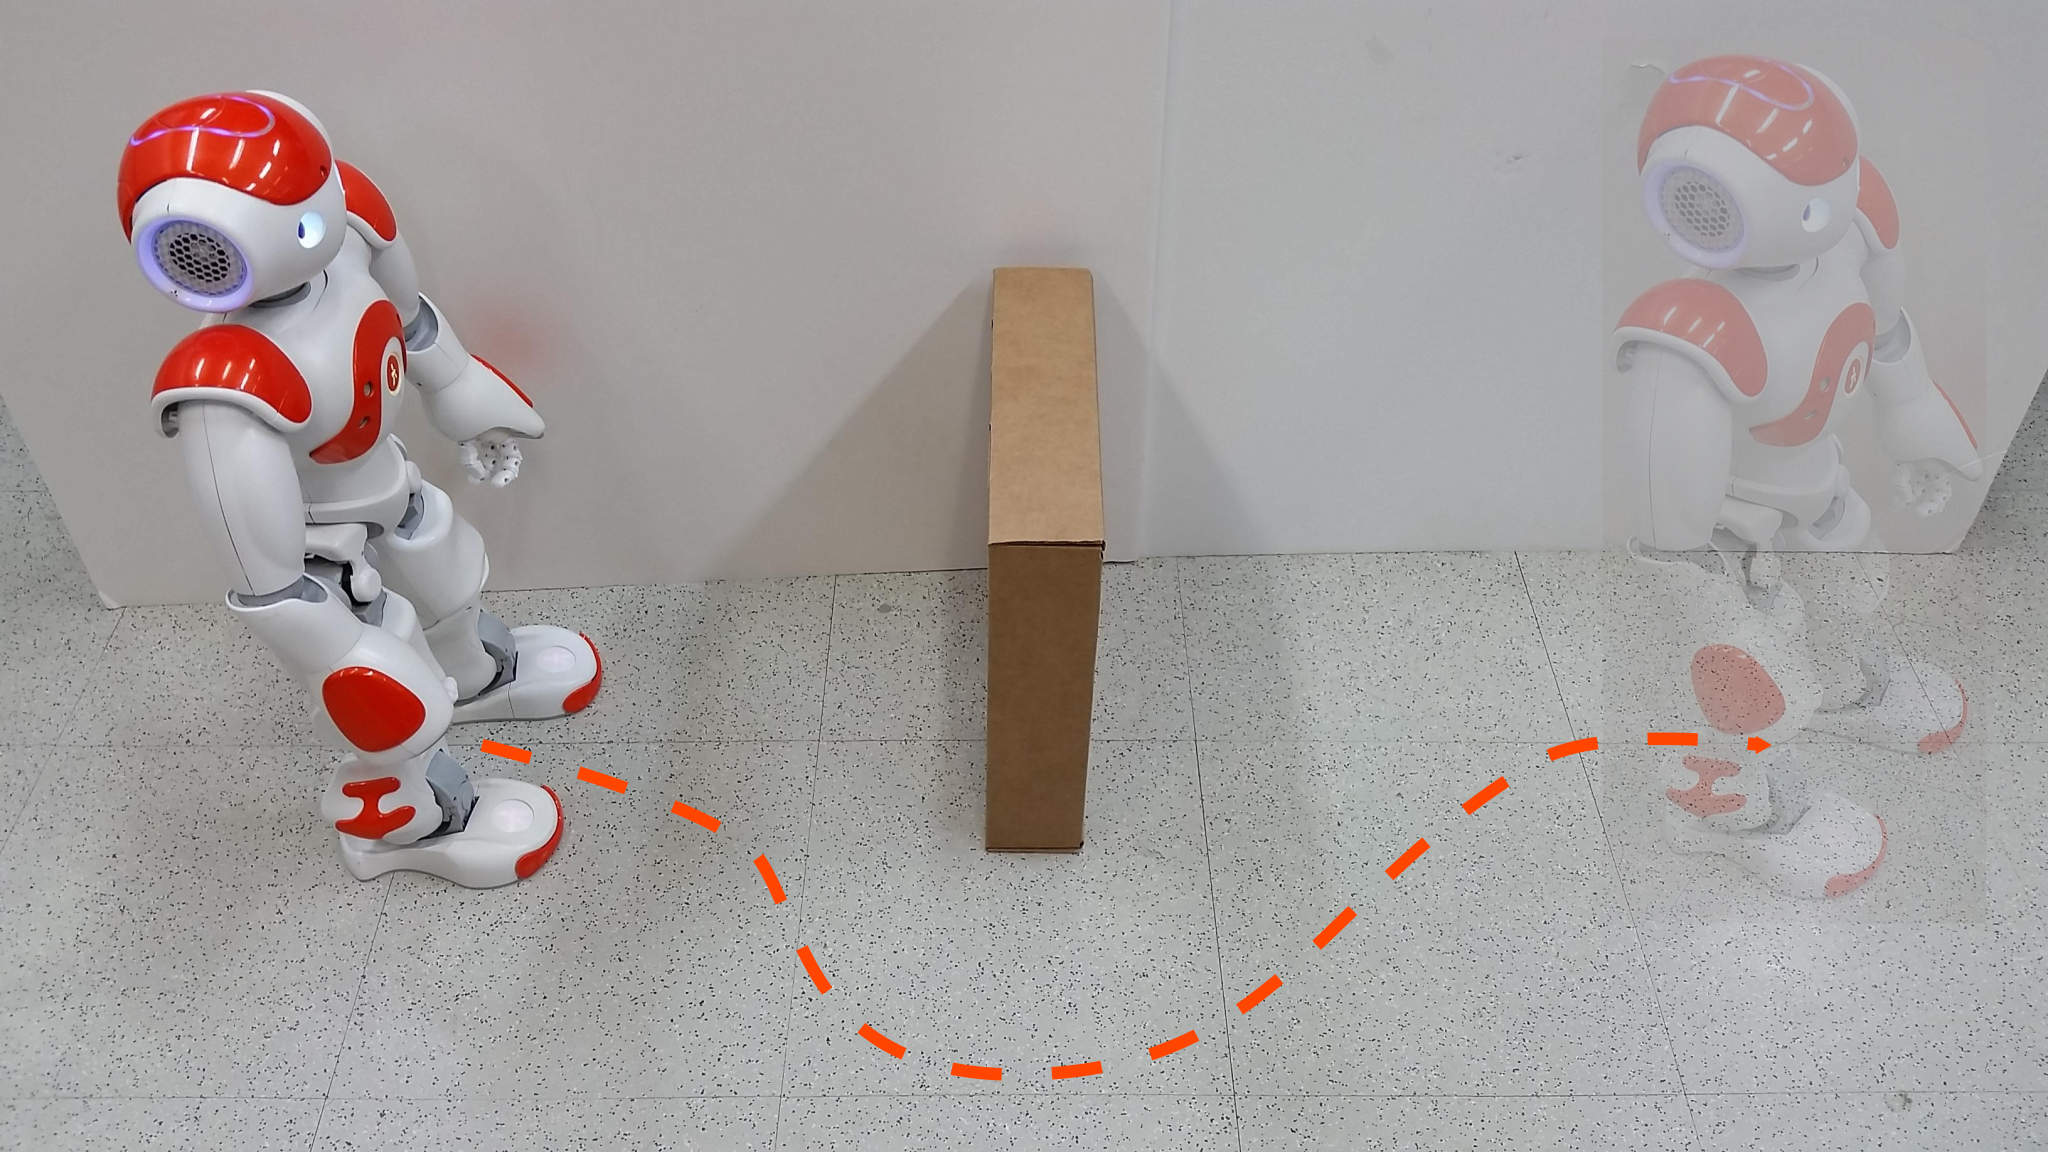
\includegraphics[width=0.7\textwidth]{nao_with_obstacle2.pdf}
	\caption{Example illustration of the Nao humanoid robot in an environment 
             with an obstacle. To reach the left side of the area,
             it must plan a path through the environment.}
	\label{fig:nao_with_obstacle2}
\end{figure}

\section{Background}
% Review previous work here as well.
% Why humanoids?
% Humanoid platforms are very adaptable. Various terrains. 
% Humanoids can locomote and manipulate.
% Humanoids are compatible with our humanoid orient environment.
% People relate to humanoids.
Humanoid robots offer a number of attractive features and interesting
challenges.
They range in size from the size of children \cite{Ishida2003, Ha2011,
Gouaillier2009, Tsagarakis2007iCubTD}, to the size of an average
adult \cite{asimo_website, atlas_website, robonaut_website, Radford2015}.
As a legged platform, it has a configuration that is adaptable 
to various terrains \cite{Iida2010, Wu2010, Lutz2012}, 
while using a minimal number of limbs to accomplish locomotion. 
In addition to being a mobile base, humanoids are also manipulators. 
This opens up possibilities for interesting interactions
with the environment \cite{levine2016, Koval2015, coleman2015}.
Humanoid platforms are also a good choice for experimenting with robots that
are expected to operate in human oriented environments as 
homes and offices are already configured to be traversable by humans.
This is showcased by competitions such as the DARPA Robotics Challenge
\cite{drc_website} and the RoboCup@Home Competitions
\cite{robocupathome_website} which both aim to further the field of robotics
toward operating in human oriented environments.
As well as being useful for navigation and manipulation, humanoid platforms
are perhaps uniquely suited for studying interactions between robots and
humans \cite{Ismail2012, Moshkina2011}. They allow for increased control
of an experiment and ensure a greater about of repeatability between
experiments.

%%% NAVIGATION %%%
% What is the problem of navigating, briefly.
% Navigation is fundamental. Get the robot somewhere safely. Otherwise it might
% as well not be mobile.
% Layered approach.
Moving a robot from one location to another in central to the problem of
mobile robotics. Navigating a mobile robot is typically implemented using
multiple approaches addressing different aspects of the problem.
% Who's done navigation?
Search-based planners, such as A* search \cite{Hart1968, gonzalez2011search,
Likhachev04ara} and Rapidly Exploring Random Trees \cite{Lavalle98rapidly} are
typically used to efficiently address global path planning, but often produce
unsmooth paths.
Planners which consider a continuous function space such as the Potential Field
algorithm \cite{ArambulaCosio2004, Koren1991, Hogan1984, Fox1997} or
Backstepping approaches \cite{Park2011, Park2015} produce smooth paths but can
have problems with complicated environments.
% We've done navigation.
The navigation algorithm used in this thesis was based on a Potential Field
approach \cite{Krishnamurthy2007}, with which we have previous experience
\cite{Brooks2013}.

%%% CRAWLING %%%
Humanoid robots have been used as a platform for exploring walking
\cite{Vukobratovic1969, Geijtenbeek2013, Deits2014}, which is important for the
field of mobile human robots. Equally important is the ability to have multiple
gaiting strategies available to traversing difficult terrain.
Humanoid crawling has been explored before in \cite{Li2011, Li_crawlingposture, 
righetti2006} and provides an interesting opportunity to expand the set of
feasible humanoid gaits \cite{Brooks2015}.

\section{Platform Overview}

\begin{figure}
	\centering
	\includegraphics[width=0.4\textwidth]{nao_coronal_highlighted2.png}
    \caption{Coronal view of the Nao humanoid with a few pertinent features 
             highlighted.}
	\label{fig:nao_diagram1}
\end{figure}

% What equipment did we use?
% - Nao
% - Lidar
% - Mount
% We used a Nao. What's that?
% We used a Lidar. What's that? We used a Hokuyo. What's that?
% We made a mount.
The mobile platform used for these experiments was the Nao H25 Humanoid
Platform from Aldebaran Robotics \cite{nao_docs_h25}. 
Figure~\ref{fig:nao_diagram1} shows the Nao at the Control/Robotics Research
Lab at NYU\@.
It is a 25 degree-of-freedom humanoid with a rich set of sensors
including cameras, sonars, joint angle sensors, and inertial measurement unit. 
It also features an onboard computer, Wifi, Ethernet, and USB 2.0. Combined with 
an extensive API, the Nao is a very capable platform, making it well suited to 
explore navigation and crawling.
To supplement the sensing capabilities of the Nao, a Hokuyo URG-04LX-UG01 
\cite{urg_specs} scanning laser rangefinder (Lidar) was mounted to the robot.
This allowed the Nao to have a high resolution survey of the local environment
that the navigation algorithm used to avoid colliding with obstacles.
% Why did we use these things?
% We used a Nao, because it's a humanoid.
% We used a Lidar because you can see more things.
% We had to make a mount to get it on there.


\section{GODZILA Navigation}
% Briefly, what's navigation?
% What approach did we go for?
% Why did we go for this?
% GODZILA is a potential field local approach.
% Potential field is this blah.
% It's cheap on memory and fast to compute.
% It's local. Now we can build more on top of it.
The navigation strategy implemented was based on the GODZILA planning algorithm
\cite{Krishnamurthy2007}. It is a local navigation strategy which produces
smooth paths. It also has a small memory footprint and is computationally 
cheap. Based on the Potential Field approach, it could serve as the foundation
that other planning algorithms build upon. While a local planner, as is shown
in Chapter~\ref{ch:navigation}, it is capable of navigating the robot through
parts of the environment which were not observable at the start of the path.

\section{Projected Profile Crawl Gait}
% Briefly, what's crawling?
% Why crawling?
% What approach did we go for?
% Why did we go for this approach?
% Statically stable.
% You take the robot as symmetric and do a saggital projection.
% Can compose the gait into two modes.
% Applicable to other platforms.
The crawling gait implemented was the Projected Profile gait \cite{Brooks2015}.
It is a statically stable crawl with two phases. In the first phase, the robot
is treated as a set of open chain manipulators, which allows the arms and feet
to be positioned independently. In the second phase, the robot forms a closed
chain, which is responsible for shifting the center-of-mass forward.
By alternating these two phases, the robot is able to crawl forward.
While implemented on a humanoid platform, this gaiting strategy is applicable
to any platform which can be viewed in this manner, such as a quadrupedal robot.

\section{Thesis Structure}
Chapter~\ref{ch:platform} reviews in detail, the design considerations for the
platform used, including the features of the Nao Humanoid Platform, Hokuyo Lidar,
and the mounting hardware designed to join the two.
% Chapter \ref{ch:navigation} discusses the GODZILA algorithm used for local navigation.
% Chapter \ref{ch:crawl_gait} discusses the Projected Profile crawling gait used to perform the crawl.
Discussion of the navigation algorithm is presented in 
Chapter~\ref{ch:navigation} while the results of the experiments are analyzed
in Chapter~\ref{ch:results_navigation}.
Formulation of the crawling gait is detailed in Chapter~\ref{ch:crawl_gait} and
both simulations and experimental results of the crawl are shown in 
Chapter~\ref{ch:results_crawl_gait}.
Finally, the performance of the algorithms are reviewed, and future work is
discussed in Chapter~\ref{ch:conclusion}.
